% ==============================================================================
% TCC - César Henrique Bernabé
% Capítulo 3 - O Unagi
% ==============================================================================

\chapter{Especificação de Requisitos}
\label{sec-requisitos}

Este capítulo aborda alguns resultados da Engenharia de Requisitos para a construção do sistema SAE. Na seção~\ref{sec-requisitos-escopo}, é apresentado o escopo do projeto; na seção~\ref{sec-requisitos-casos-de-uso}, são apresentados diagramas de casos de uso e na seção~\ref{sec-requisitos-diagrama-de-classes}, são apresentados os diagramas de classes. Os requisitos funcionais, requisitos não funcionais e regras de negócio podem ser encontrados no \textbf{Documento de Especificação de Requisitos} que está disponível no Apêndice ao final desta monografia.


\section{Descrição do Escopo}
\label{sec-requisitos-escopo}

O DI/Ufes deseja um sistema de informação para acompanhar seus alunos egressos dos cursos de graduação (Ciência da Computação e Engenharia de Computação) e de pós-graduação (Mestrado em Informática e Doutorado em Ciência da Computação). 

Para poder acessar o sistema, os egressos terão um pré-cadastro realizado por um administrador do sistema. Somente poderão ser pré-cadastrados ex-alunos que tenham se formado em algum curso oferecido pelo DI/Ufes. Para efetuar o pré-cadastro o administrador buscará os dados do egresso junto à Ufes, a saber: nome, data de nascimento, sexo, e-mail, identidade, CPF, naturalidade e nacionalidade. Também serão informados o curso em que o egresso se formou, o número de sua matrícula, o ano de ingresso e o ano de término. 

Assim que o pré-cadastro for realizado, o sistema deverá enviar um e-mail ao egresso com um link que o leva diretamente para uma página onde pode definir sua senha. Para aumentar a segurança, esta página solicita o CPF ou a matrícula do egresso para efetivar a definição de senha. Caso o egresso perca este e-mail, poderá receber outro, devendo para isso entrar no site e informar o seu CPF/matrícula. Reconhecendo o egresso, o sistema enviará o e-mail.
 
Assim que for criada a senha, o sistema levará o egresso a uma página onde ele preencherá um formulário com os seguintes campos: faixa salarial, área de atuação, se atua na área em que se formou, nível de escolaridade e se reside no ES. Para cada nível de escolaridade deve dizer o título obtido, o ano, a instituição, o estado e o país.

O tempo médio exigido para o preenchimento deste formulário deve ser inferior a 5 minutos. A cada 2 anos o sistema deverá enviar um e-mail para que o usuário atualize esses dados, sendo armazenado o histórico dos mesmos.

Os egressos escolherão a sua área de atuação dentre as seguintes opções: empreendedor; funcionário público; funcionário privado; professor; ou pesquisador. E informarão se atuam em Informática, área afim ou área não correlata. Será perguntado se a formação acadêmica adquirida no curso da Ufes contribuiu para a sua atividade atual.

Os egressos escolherão a faixa salarial, dividida da seguinte forma: até 3 salários mínimos; de 3 a 5 salários mínimos; de 5 a 10 salários mínimos;  de 10 a 15 salários mínimos; de 15 a 20 salários mínimos; e acima de 20 salários mínimos. Poderão também optar por assuntos de interesse para recebimento de e-mail. A princípio os assuntos serão: Redes de Computadores e Sistemas Distribuídos; Computação de Alto Desempenho; Inteligência Computacional; Sistema de Informação; e Otimização. 

Egressos poderão postar depoimentos sobre o curso que realizaram. Esses depoimentos ficarão acessíveis a todos que acessarem o site, depois de serem avaliados e liberados pelo coordenador do curso a fim de evitar críticas gratuitas depreciativas. O egresso poderá optar por aparecer seu nome no depoimento ou se ele quer que fique anônimo. De um depoimento deseja-se saber a data de envio, sobre qual curso, o autor e o conteúdo. 

Assim como no caso dos depoimentos, os egressos também poderão mandar comentários ou sugestões sobre o curso que realizaram. Estes serão enviadas para o coordenador do curso para que possa respondê-los e também auxiliar em melhorias a serem feitas nos cursos. 

Administradores do sistema poderão cadastrar seminários, informando o assunto, o título, a data e horário, o local e o palestrante. Caso não tenha palestrante ainda, o administrador terá a opção de enviar um e-mail aos egressos convidando-os a serem o palestrante. Caso alguém responda ao chamado (por e-mail, externo ao sistema), o administrador terminaria o cadastro do seminário. Assim que a palestra estiver confirmada, o sistema enviará um e-mail para todos os egressos que tenham interesse pelo assunto, convidando-os para participarem. Os egressos também teriam a opção de sugerir um assunto em que tenham interesse em ser o palestrante. Neste caso o administrador confirmaria com ele e cadastraria o seminário no sistema.


No site, ficarão disponíveis para consulta relatórios sobre dados estatísticos. Estes dados serão mostrados na forma de gráficos, assim os usuários poderão escolher um curso e optar pelos seguintes gráficos: 

\begin{itemize}
	
  	\item \textbf{Faixa Salarial:} mostra a porcentagem de egresso em cada faixa salarial.
  	
  	\item \textbf{Área de Atuação:} mostra a porcentagem de egresso em cada área: (Empreendedor), (Func. Público), (Func. Privado), (Professor) e (Pesquisador).
  	
  	\item \textbf{Atuação do Egresso:} mostra a porcentagem de egressos que atuam na área da informática, a porcentagem dos que atuam em áreas afins e a porcentagem dos que atuam em áreas não correlatas. 
  	
  	\item \textbf{Escolaridade:} mostra a porcentagem de egressos em cada nível de escolaridade. 
  	
  	\item \textbf{Reside no ES:} mostra a porcentagem de egressos que moram no Estado.
  	
  	\item \textbf{Sexo:} mostra a porcentagem de egressos do sexo masculino e feminino.
  	  	
\end{itemize}

Os usuários também poderão consultar todos os egressos, que serão mostrados na forma de lista. 











%%% Início de seção. %%%
\section{Diagrama de Casos de Uso}
\label{sec-requisitos-casos-de-uso}
	
Este projeto foi divido em dois subsistemas \texttt{sae.core} e \texttt{sae.public}, sendo que o subsistema \texttt{sae.core} envolve toda a funcionalidade relacionada com o administrador do sistema, abrangendo controle de seminários, cursos, assuntos de interesse, envio de e-mail automático e pré-cadastro de egresso. O subsistema \texttt{sae.public} envolve toda a funcionalidade relacionada com consultas a serem realizadas no site, e com as interações que os egressos poderão fazer, tais como cadastrar depoimentos e sugestões.
Veremos na Subseção~\ref{sec-requisitos-casos-de-uso-core} os casos de uso do subsistema \texttt{sae.core} e na Subseção~\ref{sec-requisitos-casos-de-uso-public} os casos de uso do subsistema \texttt{sae.public}.
	
	
	
\subsection{Atores}
\label{sec-requisitos-casos-de-uso-atores}
O modelo de casos de uso visa capturar e descrever as funcionalidades que um sistema deve prover para os atores que interagem com o mesmo. A Tabela~\ref{tabela-atores} descreve cada um dos atores identificados no sistema.


	
\begin{table}[h]
	\centering \vspace{0.5cm} \caption{ Atores}
	\begin{tabular}{|p{3cm}|p{12cm}|} \hline \rowcolor[rgb]{0.8,0.8,0.8}
 		Ator & Descrição \\\hline                              
		Administrador & Profissional da Ufes responsável pela parte administrativa do sistema. \\\hline   
		Coordenador & É um administrador responsável por um curso, avaliando depoimentos e sugestões enviadas pelos egressos. \\\hline                              
		Egresso & Ex-alunos da Ufes que tenham se formado em algum curso oferecido pelo DI/Ufes. \\\hline                              
		Visitante & Qualquer pessoa que acessar o site. \\\hline 		 
	\end{tabular}
	\label{tabela-atores}	
\end{table}

	
A Figura~\ref{fig-requisitos-diagrama-atores} apresenta o diagrama de herança entre os atores do sistema, de modo que essas heranças não serão mostradas nos outros diagramas para evitar a poluição visual.
\begin{figure}[h]
	\centering
	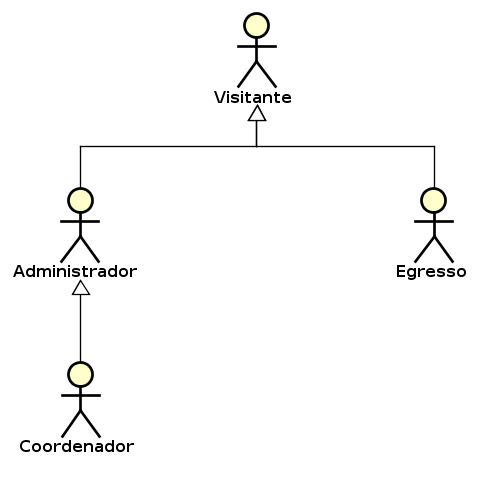
\includegraphics[width=0.35\textwidth]{figuras/requisitos/atoresHeranca}
	\caption{SAE - CORE - Diagrama de Casos de Uso.}
	\label{fig-requisitos-diagrama-atores}
\end{figure}

	
\newpage	
\subsection{Subsistema sae.core}
\label{sec-requisitos-casos-de-uso-core}

A Figura~\ref{fig-requisitos-core-diagrama-casos-uso} mostra os casos de uso do subsistema \textbf{\texttt{sae.core}} que serão descritos a seguir. O subsistema \textbf{\texttt{sae.core}} foi criado para gerenciar as funcionalidades que só os administradores podem realizar. Os casos de uso \textbf{Gerenciar Cursos, Gerenciar Administradores, Gerenciar Egressos, Gerenciar Assuntos de Interesse e Gerenciar Seminário } são do tipo cadastrais e incluem alteração, inclusão, consulta e exclusão. 

\begin{figure}[h]
	\centering
	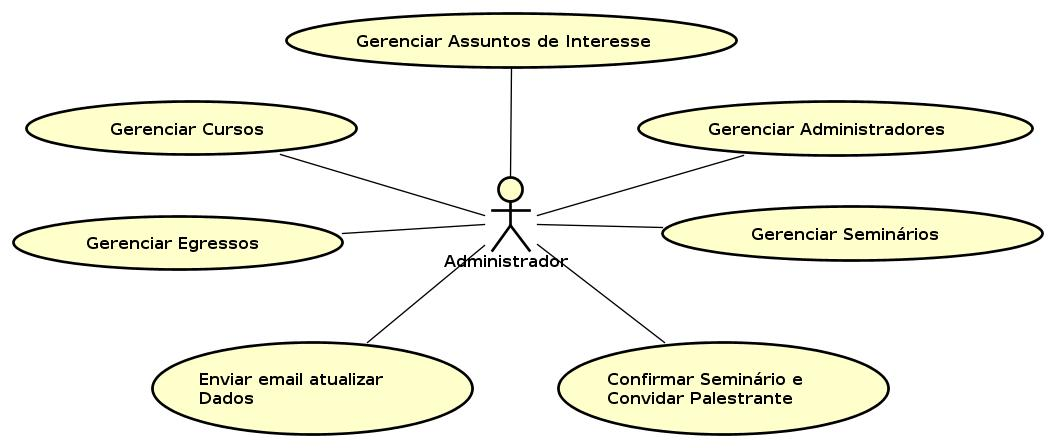
\includegraphics[width=0.95\textwidth]{figuras/requisitos/casodeuso-core}
	\caption{SAE - CORE - Diagrama de Casos de Uso.}
	\label{fig-requisitos-core-diagrama-casos-uso}
\end{figure}

O DI/Ufes possui cursos de graduação e de pós-graduação. Então, foi criado o caso de uso \textbf{Gerenciar Cursos} para que o administrador possa inserir novos cursos, possa também consultar, alterar e até mesmo excluir um curso. Para inserir um novo curso, basta informar o código, o nome e o coordenador do curso.

Uma informação crucial para o sistema são os Administradores, que serão controlados pelo caso de uso \textbf{Gerenciar Administradores}. Nesse caso, deve ser informado: nome, e-mail (será o login para acessar o sistema), CPF e matricula.

Os egressos são uma das partes fundamentais do sistema, assim serão controlados pelo caso de uso \textbf{Gerenciar Egresso}. As informações necessárias de um egresso são: nome, e-mail (será o login para acessar o sistema), data de nascimento, sexo, identidade, CPF, naturalidade e nacionalidade, também são necessários informar o curso, a matrícula, o ano de início e de término do curso.  

Os egressos poderão escolher assuntos de interesse para recebimento de e-mail. A princípio os assuntos serão: Redes de Computadores e Sistemas Distribuídos; Computação de Alto Desempenho; Inteligência Computacional; Sistema de Informação; e Otimização. Assim foi criado o caso de uso \textbf{Gerenciar Assuntos de Interesse} para realizar esse controle. A informação de um assunto é o nome.


Seminários também poderão ser cadastrados no sistema. Assim teremos os casos de uso \textbf{Gerenciar Seminário}, \textbf{Confirmar Seminário} e \textbf{Convidar Palestrante} para fazer o controle. O caso de uso  \textit{Gerenciar Seminário} será cadastral, enquanto o  \textit{Confirmar Seminário e Convidar Palestrante} envolve atividades como enviar e-mail a todos os egressos que tenham interesse no assunto do seminário assim que este for confirmado, enviar e-mail aos egressos convidando a serem o palestrante de seminário cujo assunto é de seu interesse.

Para manter os dados dos egressos atualizados será enviado, a cada 2 anos, um e-mail para todos os egressos solicitando que estes façam a atualização de seus dados. O caso de uso \textbf{Enviar e-mail atualizar dados} será responsável por este envio de e-mail.
	
	
	






\subsection{Subsistema sae.public}
\label{sec-requisitos-casos-de-uso-public}
 

A Figura~\ref{fig-requisitos-public-diagrama-casos-uso} mostra os casos de uso do subsistema \textbf{\texttt{sae.public}} que serão descritos abaixo. Este subsistema foi criado para gerenciar as funcionalidades relacionadas com consultas a serem realizadas no site e com as interações que os egressos poderão fazer, tais como cadastrar depoimentos e sugestões através dos casos de uso \textbf{Gerenciar Depoimentos, Gerenciar Sugestões, Gerenciar Escolaridades e Gerenciar Históricos}. Os casos de uso de consulta são \textbf{Consultar Todos Egressos, Consultar Depoimento e Consultar dados Estatísticos}, que poderão ser realizado por qualquer usuário do sistema. 

\begin{figure}[!h]
	\centering
	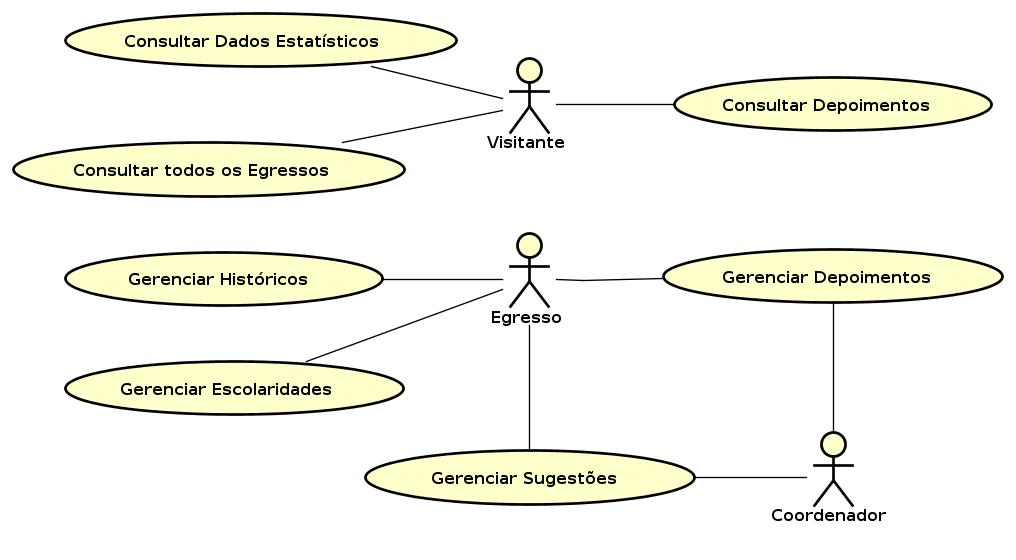
\includegraphics[width=1\textwidth]{figuras/requisitos/casodeuso-public}
	\caption{SAE - PUBLIC - Diagrama de Casos de Uso.}
	\label{fig-requisitos-public-diagrama-casos-uso}
\end{figure}

No caso de uso \textbf{Consultar Todos Egressos} as consultas poderão ser feitas de forma geral onde serão mostrados todos os egressos, ou por curso, onde serão mostrados apenas os egressos que formaram naquele curso. Será exibido na tela para ao usuário o nome do egresso, o curso que realizou, o ano de início e o ano de término.

No caso de uso \textbf{Consultar Depoimento} as consultas aos depoimentos poderão ser realizadas de forma geral onde serão mostrados todos os depoimentos, ou por curso, onde serão mostrados apenas depoimentos sobre o curso escolhido. Será exibido na tela o conteúdo, o autor e a data de postagem. Somente serão mostrados nesta consulta depoimentos que tenham sido analisados e aprovados pelo coordenador do curso que se refere o depoimento.

No caso de uso \textbf{Consultar dados Estatísticos} as consultas serão feitas com bases nos dados mais atuais dos egressos. Alguns exemplos de gráficos que poderão ser gerados nesta consulta são \textit{Faixa Salarial, Área de Atuação, Escolaridade e Sexo}.
  	  
Egressos poderão postar depoimentos sobre o curso que realizaram. Esses depoimentos ficarão acessíveis a todos que acessarem o site, depois de serem avaliados e liberados pelo coordenador do curso a fim de evitar criticas gratuitas depreciativas, assim foi criado o caso de uso \textbf{Gerenciar Depoimentos} para fazer esse controle.  

Assim como no caso dos depoimentos, os egressos também poderão mandar comentários ou sugestões sobre o curso que realizaram. Estes serão enviadas para o coordenador do curso para que possa respondê-los o caso de uso responsável por fazer esse controle é \textbf{Gerenciar Sugestões}.


No caso de uso \textbf{Gerenciar Históricos} o egresso informará sua faixa salarial, área de atuação que pode ser funcionário no setor público ou no setor privado, empreendedor, professor ou pesquisador, informará também se atua na área da informática, se reside no Espirito Santo e o seu maior nível de escolaridade. Com essas informações será possível criar o perfil dos egressos.


No caso de uso \textbf{Gerenciar Escolaridades} o egresso poderá cadastrar todos seus cursos realizados a nível de graduação, especialização, mestrado, doutorado ou pós-doutorado. Para cada curso ele informará a instituição, o estado e o país, e o ano de conclusão.


Maiores informações e detalhes sobre os casos de uso poderão ser consultados no \textbf{Documento de Análise de Requisitos} que está disponível no Apêndice ao final dessa monografia.






%%% Início de seção. %%%
\section{Diagrama de Classes}
\label{sec-requisitos-diagrama-de-classes}


Assim como os casos de uso na seção~\ref{sec-requisitos-casos-de-uso} os diagramas de classes estão dividos de acordo com a divisão dos subsistemas, na Subseção~\ref{sec-requisitos-diagrama-de-classes-core} estão as classes pertecentes ao subsistema \texttt{sae.core} e na Subseção~\ref{sec-requisitos-diagrama-de-classes-public} estão as classes pertencentes ao subsistema \texttt{sae.public}.



\subsection{Subsistema sae.core}
\label{sec-requisitos-diagrama-de-classes-core}

A Figura~\ref{fig-requisitos-core-diagrama-classes} exibe o diagrama de classes do subsistema \textbf{\texttt{sae.core}}. Uma das classes mais importante é a \textbf{Egresso} que possui ligações com outras classes tanto no subsistema \textit{\texttt{sae.core}} quanto no subsistema \textit{\texttt{sae.public}}. É obrigatório que um \emph{egresso} possua um \emph{curso}, que será feito através da classe \textbf{Curso Realizado} visto que para ser egresso do DI/Ufes é preciso ter realizado um curso. Entretanto é opcional um \emph{egresso} ter um \emph{assunto de interesse}, podendo ter mais de um.

\begin{figure}[h]
	\centering
	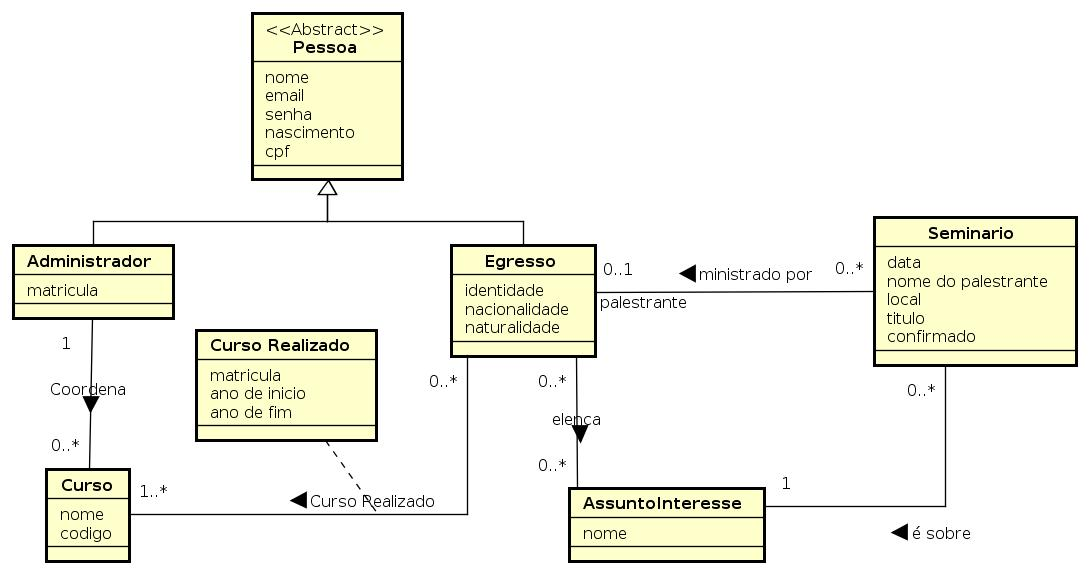
\includegraphics[width=1\textwidth]{figuras/requisitos/diagrama-classe-core}
	\caption{SAE - CORE - Diagrama de Classes.}
	\label{fig-requisitos-core-diagrama-classes}
\end{figure}

As classes \textbf{Administrador} e \textbf{Assunto de Interesse} podem ter registros no sistema e mesmo assim não estarem ligadas a nenhuma outra classe. Todo \emph{curso} deve ter um \emph{administrador} associado a ele, visto que este desempenhará o papel de coordenador do curso, sendo responsável por avaliar depoimento e responder sugestões do curso que coordena. Um \emph{seminário} precisa ter, obrigatoriamente, um \emph{assunto de interesse}.



\subsection{Subsistema sae.public}
\label{sec-requisitos-diagrama-de-classes-public}

A Figura~\ref{fig-requisitos-public-diagrama-classes} exibe o diagrama de classes do subsistema \textbf{\texttt{sae.public}}. Podemos notar que as classes \textbf{Egresso} e \textbf{Curso} foram referenciadas do subsistema \texttt{sae.core}. Portanto, fazem parte desse subsistema as classes \textbf{Depoimento}, \textbf{Sugestão}, \textbf{Escolaridade} e \textbf{Histórico do Egresso}. Uma \emph{escolaridade} e um \emph{histórico do egresso} devem estar associados a um \emph{egresso}. Um \emph{depoimento} e uma \emph{sugestão}, além de um \emph{egresso}, também devem ter um \emph{curso} associado a eles.

\begin{figure}[h]
	\centering
	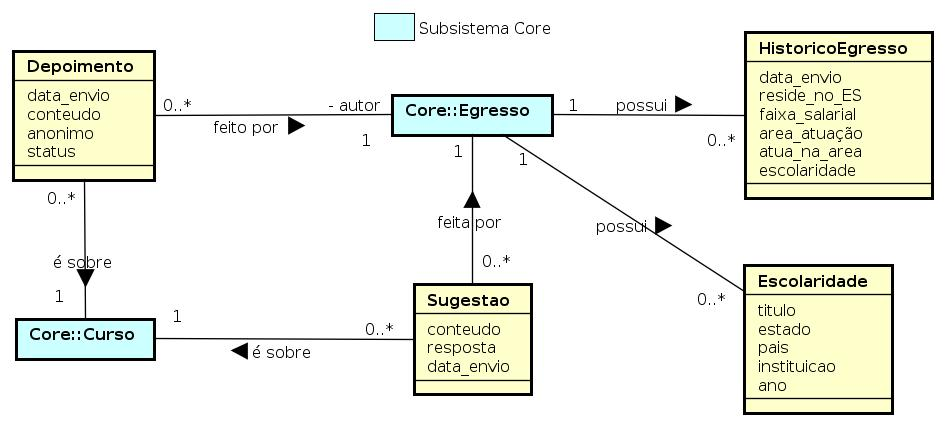
\includegraphics[width=1\textwidth]{figuras/requisitos/diagrama-classe-public}
	\caption{SAE - PUBLIC - Diagrama de Classes.}
	\label{fig-requisitos-public-diagrama-classes}
\end{figure}


Esse diagrama possui uma única restrição de integridade: uma sugestão feita por um egresso deve ser sobre um curso que este egresso tenha realizado, o mesmo vale para a classe \textbf{Depoimento}.

Maiores informações sobre o diagrama de classes poderão ser consultados no Documento de Especificação de Requisitos, disponível no Apêndice ao final dessa monografia.